\documentclass[conference]{IEEEtran}
\usepackage{cite}
\usepackage{amsmath,amssymb}
\usepackage{float}
\usepackage{graphicx}
\usepackage{xcolor}
\usepackage{hyperref}

\begin{document}

\title{Cloud Infrastructure With Confidential Computing}

\author{
    \IEEEauthorblockN{Kelan Morgan}
    \IEEEauthorblockA{
        Cloud Computing \\
        South East Technological University \\
        4th Year Software Deveolpment
    }
}

\maketitle

\begin{abstract}
As cloud computing becomes more and more important to software infrastructure, 
ensuring the security of sensitive data while in use—not just at rest or in transit—has emerged 
as a critical concern. Confidential Computing is an emerging practice that addresses this challenge 
through the use of Trusted Execution Environments (TEEs), which offer hardware-based isolation for 
data and computation. Examples of such TEEs include Intel SGX\cite{intelSGX}, AMD SEV\cite{amdSEV}, 
and ARM TrustZone\cite{armTrustZone}. This paper 
explores the motivation behind Confidential Computing, provides a technical overview of its 
architecture, and examines real-world use cases in sectors such as finance and AI workloads. 
We assess 
its practical implications and performance-security trade-offs using case studies, and discuss the 
current limitations and future challenges in deploying Confidential Computing across cloud environments.
\end{abstract}

\section{Introduction}
Cloud computing has revolutionized how organizations store, process, and manage data. However, 
as more sensitive data and worklods move over to public clouds which are easly accessed, 
there are increased concerns around data 
confidentiality, particularly during processing, have increased a lot. Traditional security measures 
such as encryption while it is stored and traveling across the network 
are becoming insufficient insufficient for protecting data in use — such as, 
data being processed in memory. This gap has driven the development of Confidential Computing, 
a important new part of cloud infrastructure aiming to ensure data remains protected throughout its 
entire lifecycle.

This report explores the architecture, existing and very impressive technologies, and practical 
implications of Confidential Computing in cloud environments. The goal is to provide a comprehensive 
overview accessible to those familiar with general cloud computing principles but not necessarily 
versed in secure hardware or cryptographic techniques.

This report contains the following:

1. Explaination of the concept of Confidential Computing and its enabling technologies.

2. comparative analysis of major Confidential Computing platforms and cloud provider offerings.

3. use cases and identification of limitations that need to be addressed for broader adoption.

\section{Related Work}
Confidential computing is a relatively new but growing field in cloud security. 
It builds on early work involving TEEs like Intel Software Guard Extensions (SGX), 
which provides per-process enclaves that isolate code and data from other applications and the OS 
\cite{intelSGX}. In parallel, AMD's Secure Encrypted Virtualization (SEV) extends protection to 
full virtual machines with memory encryption and isolation at the hypervisor level \cite{amdSEV}. 
ARM's TrustZone offers a system-level secure world used in mobile and embedded systems 
\cite{armTrustZone}.

Some of the most important contributions where previded by academics such as Costan and Devadas’ 
seminal paper “Intel SGX Explained” which provided a 
comprehensive analysis of SGX's strengths and limitations \cite{costan2016intel}. Arnautov et al. 
proposed SCONE, a secure container framework built on top of SGX, which integrates well with 
containerized applications while maintaining performance \cite{arnautov2016scone}.

Security concerns still persist. Research such as Foreshadow has shown that SGX enclaves can be 
vulnerable to transient execution attacks like speculative side channels \cite{van2018foreshadow}. 
To mitigate these, additional hardware and microcode updates are required, but vulnerabilities 
remain 
a pressing concern for real-world deployment.

Recent industry initiatives such as the Confidential Containers (CoCo) project under the Cloud 
Native Computing Foundation aim to extend TEEs to Kubernetes workloads, enabling confidential 
container deployment across multiple cloud providers \cite{coco}.

\subsection{Advancements in Confidential Computing for Machine Learning}
The integration of confidential computing with machine learning (ML) has garnered significant 
attention, particularly in scenarios involving sensitive data processing across distributed 
environments. A survey by Zobaed and Salehi explores the deployment of Trusted Execution 
Environments (TEEs) in edge-to-cloud infrastructures, emphasizing their role in securing ML 
workflows \cite{machine_learning}. The study highlights the necessity for robust attestation 
mechanisms and addresses 
challenges related to performance overheads and the complexity of managing TEEs in heterogeneous 
systems.

\section{System Architecture}
Confidential computing architecture is designed to protect data in use by performing computations 
within hardware-based Trusted Execution Environments (TEEs). The core components of this 
architecture include TEEs, remote attestation services, and secure runtime environments.

\subsection{Trusted Execution Environments (TEEs)}
TEEs provide isolated environments that ensure the confidentiality and integrity of code and 
data during execution. Examples include Intel Software Guard Extensions (SGX), AMD Secure Encrypted 
Virtualization (SEV), and ARM TrustZone. These technologies enable secure execution by isolating 
sensitive computations from the rest of the system.

\subsection{Remote Attestation Services}
Remote attestation is a process that verifies the integrity of the TEE before 
sensitive data is processed. It ensures that the code running inside the TEE has not been 
tampered with and is running in a secure environment. This is crucial for establishing trust in 
cloud and distributed systems. Tools like Gramine, Veraison, and Keylime facilitate remote 
attestation across various platforms \cite{remote_attestation}. 

\subsection{Secure Runtime Environments}
Secure runtime environments, such as Kata Containers, are lightweight virtual 
machines that provide an additional layer of isolation. In Kubernetes environments, 
these containers are launched as pods and wrapped in TEEs using frameworks like Confidential 
Containers (CoCo). This setup allows for secure deployment and execution of containerized 
applications \cite{secure_runtime_environments}. 

\begin{figure}[H]
\centerline{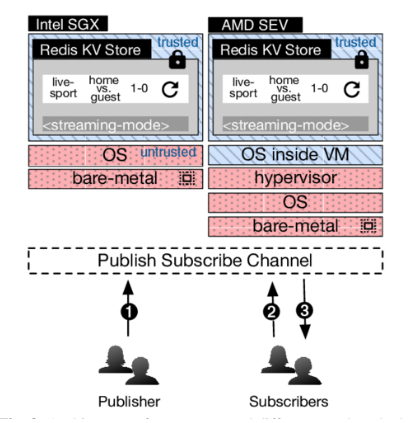
\includegraphics[width=\linewidth]{figures/architecture.png}}
\caption{Confidential Computing Architecture with Intel SGX and AMD SEV. Source: \cite{researchgate_architecture}}
\label{fig:architecture}
\end{figure}

\subsection{Attestation Process in Confidential Containers}
In the context of confidential containers, the attestation process involves verifying the 
container runtime stack running within the confidential environment. This includes components 
like the kata-agent and supporting services \cite{secure_runtime_environments}. The process ensures that both the virtual machine 
and the container runtime components are trustworthy before sensitive workloads are executed \cite{remote_attestation}. 

\begin{figure}[H]
\centerline{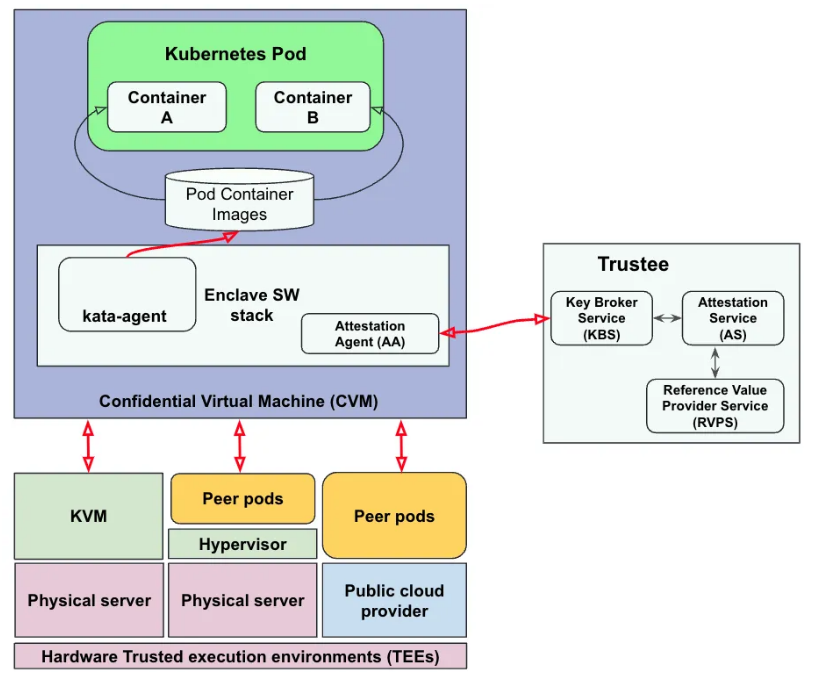
\includegraphics[width=\linewidth]{figures/attestation_process.png}}
\caption{Attestation Process in Confidential Containers. Source: \cite{redhat_attestation}}
\label{fig:attestation}
\end{figure}

\subsection{Pod-Centric Approach in Confidential Containers}
Confidential Containers adopt a pod-centric approach, balancing the Trusted Computing Base (TCB) 
size and resource sharing. This method places the workload pod and necessary helper processes 
within the enclave, while keeping other components like the hypervisor and control plane outside. 
This design enhances security while maintaining efficient resource utilization \cite{coco_architecture}.

\begin{figure}[H]
\centerline{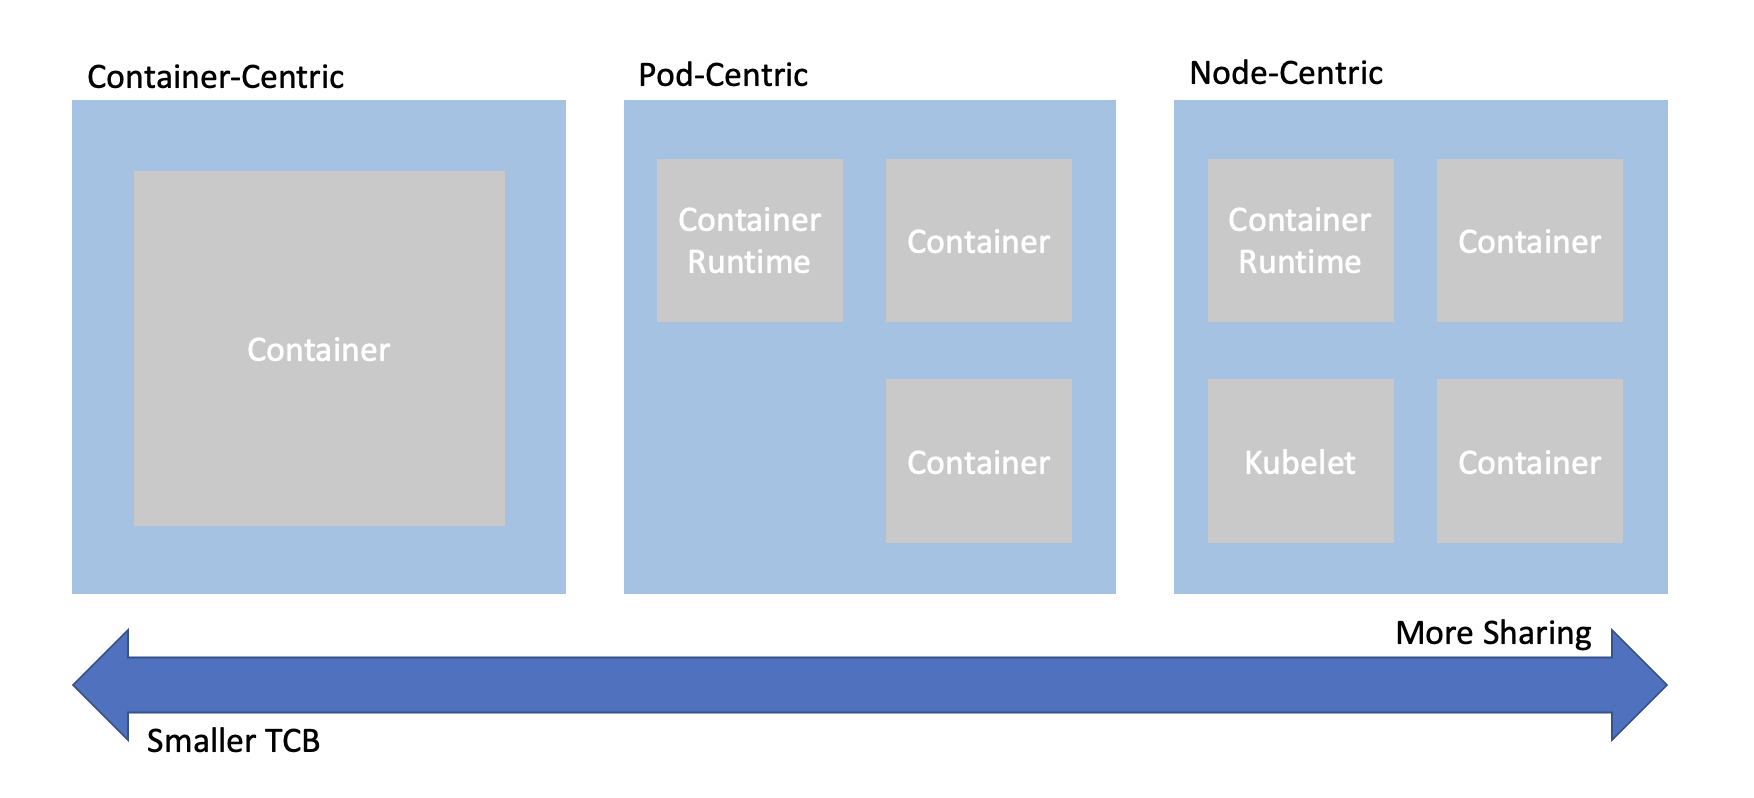
\includegraphics[width=\linewidth]{figures/pod_centric_architecture.png}}
\caption{Pod-Centric Architecture in Confidential Containers. Source: \cite{coco_architecture}}
\label{fig:pod_centric}
\end{figure}

\section{Use Cases}
Confidential computing is particularly beneficial in scenarios involving sensitive data, 
multi-party collaboration, or stringent regulatory requirements. By leveraging Trusted Execution 
Environments (TEEs), organizations can ensure data confidentiality and integrity during processing.

\begin{figure}[H]
\centerline{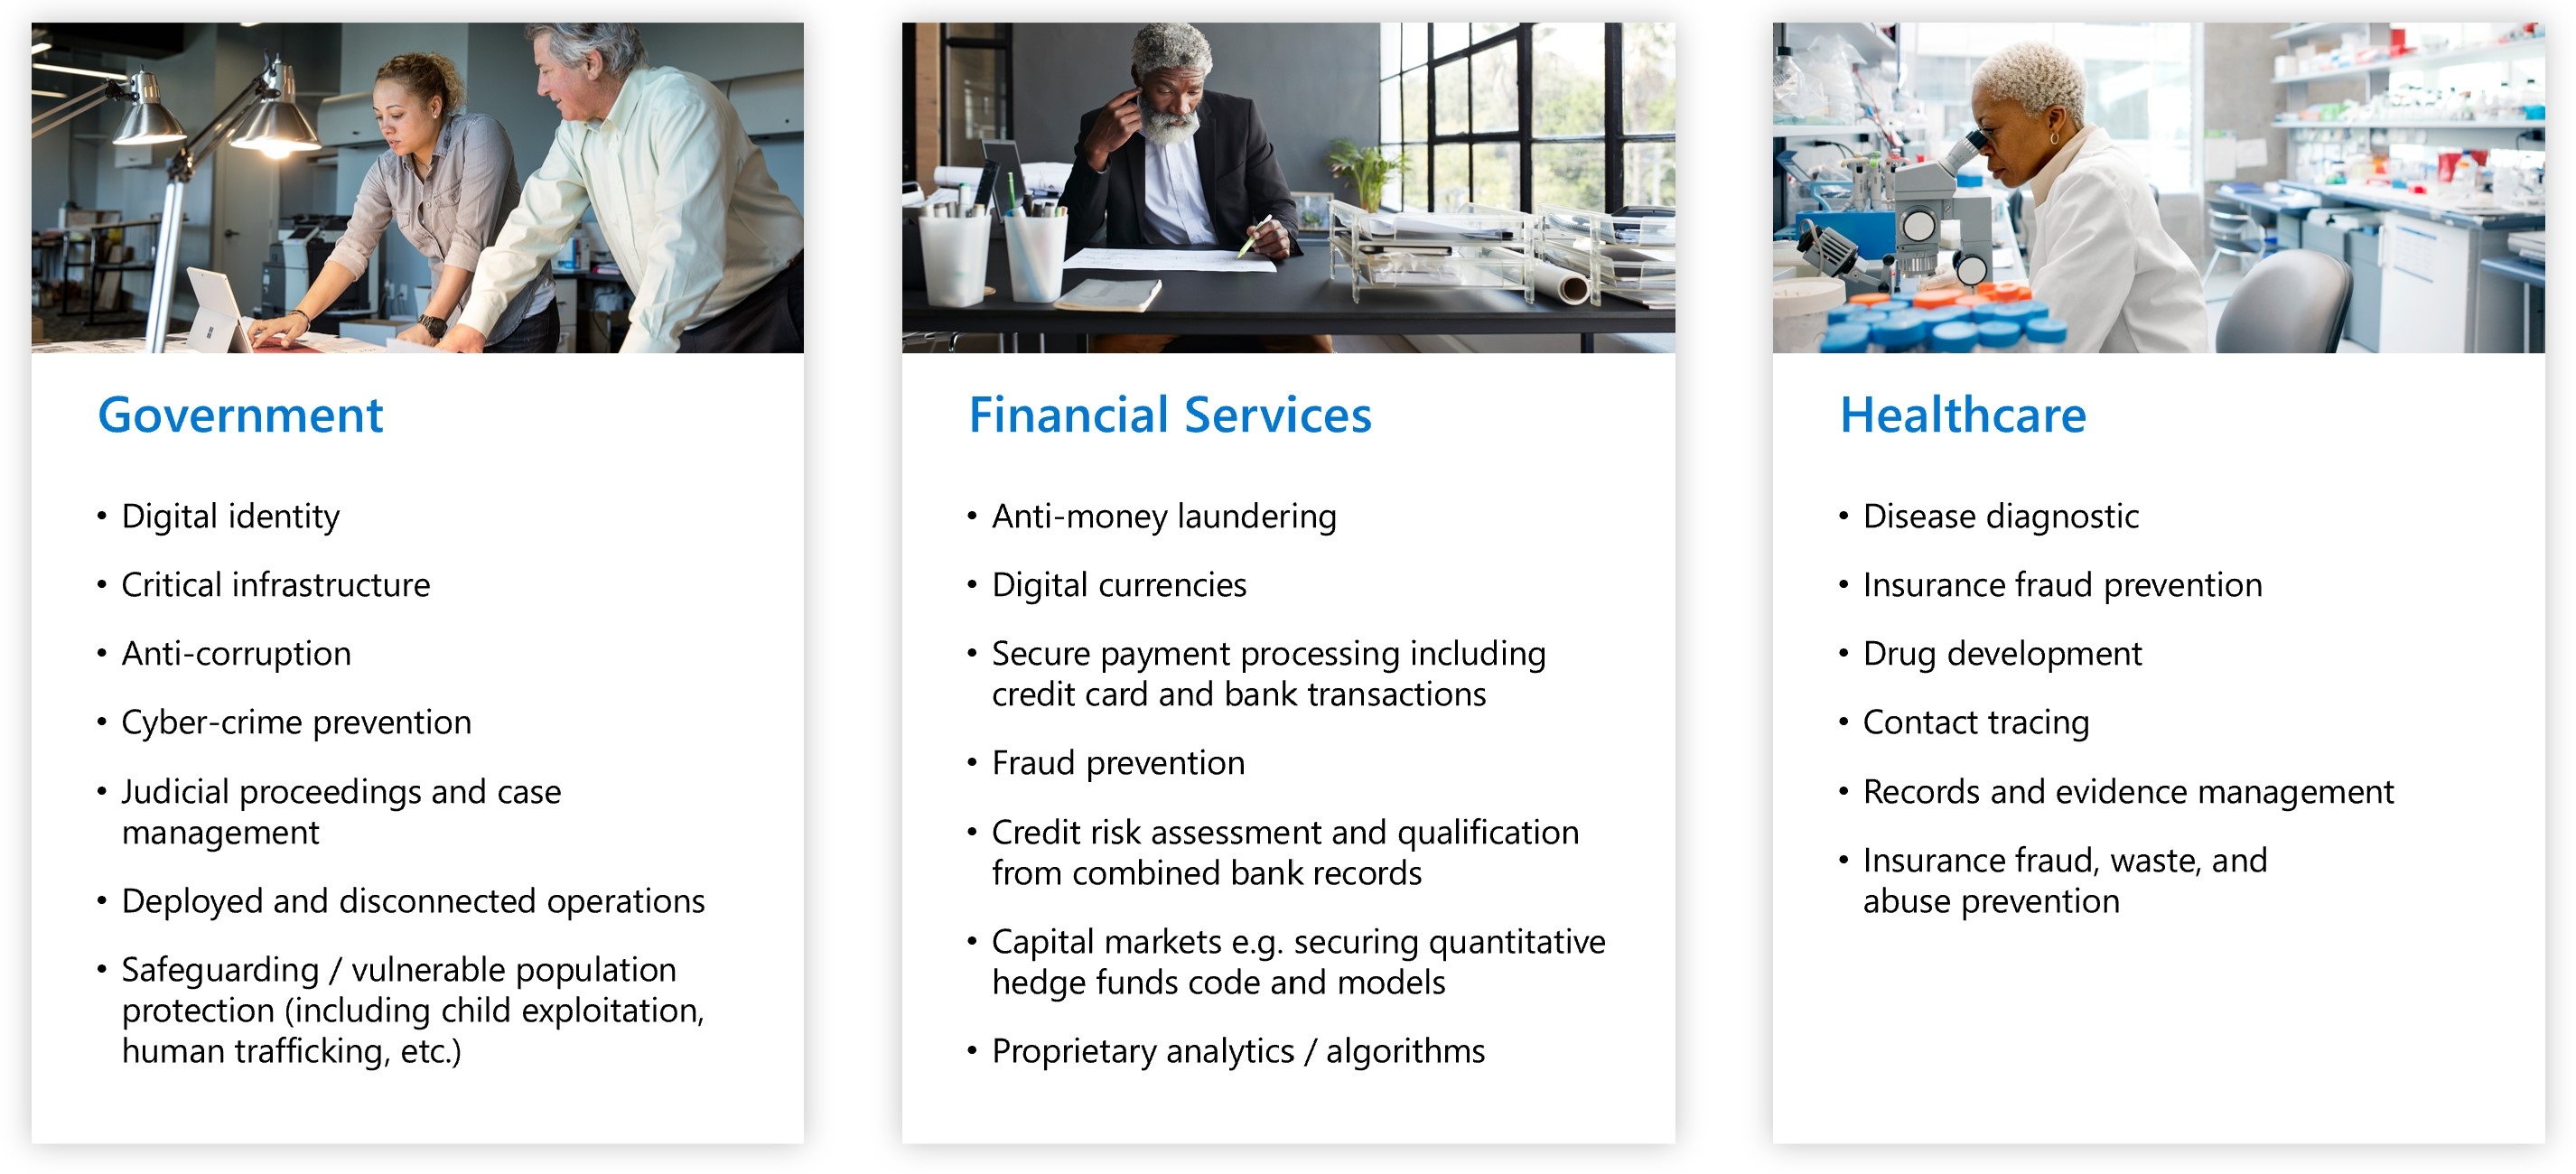
\includegraphics[width=\linewidth]{figures/mpc-uses.png}}
\caption{Secure Multi-Party Computation in Banking. Source: \cite{azure_mpc}}
\label{fig:mpc_banking}
\end{figure}

A. Secure Multi-Party Computation
Multiple institutions, such as banks or healthcare organizations, can collaboratively analyze 
data without exposing their individual datasets. For instance, in anti-money laundering (AML) 
efforts, banks can share encrypted transaction data within a secure enclave to detect fraudulent 
activities without revealing customer information. This approach enhances fraud detection while 
maintaining data privacy \cite{azure_edge}.

\begin{figure}[H]
\centerline{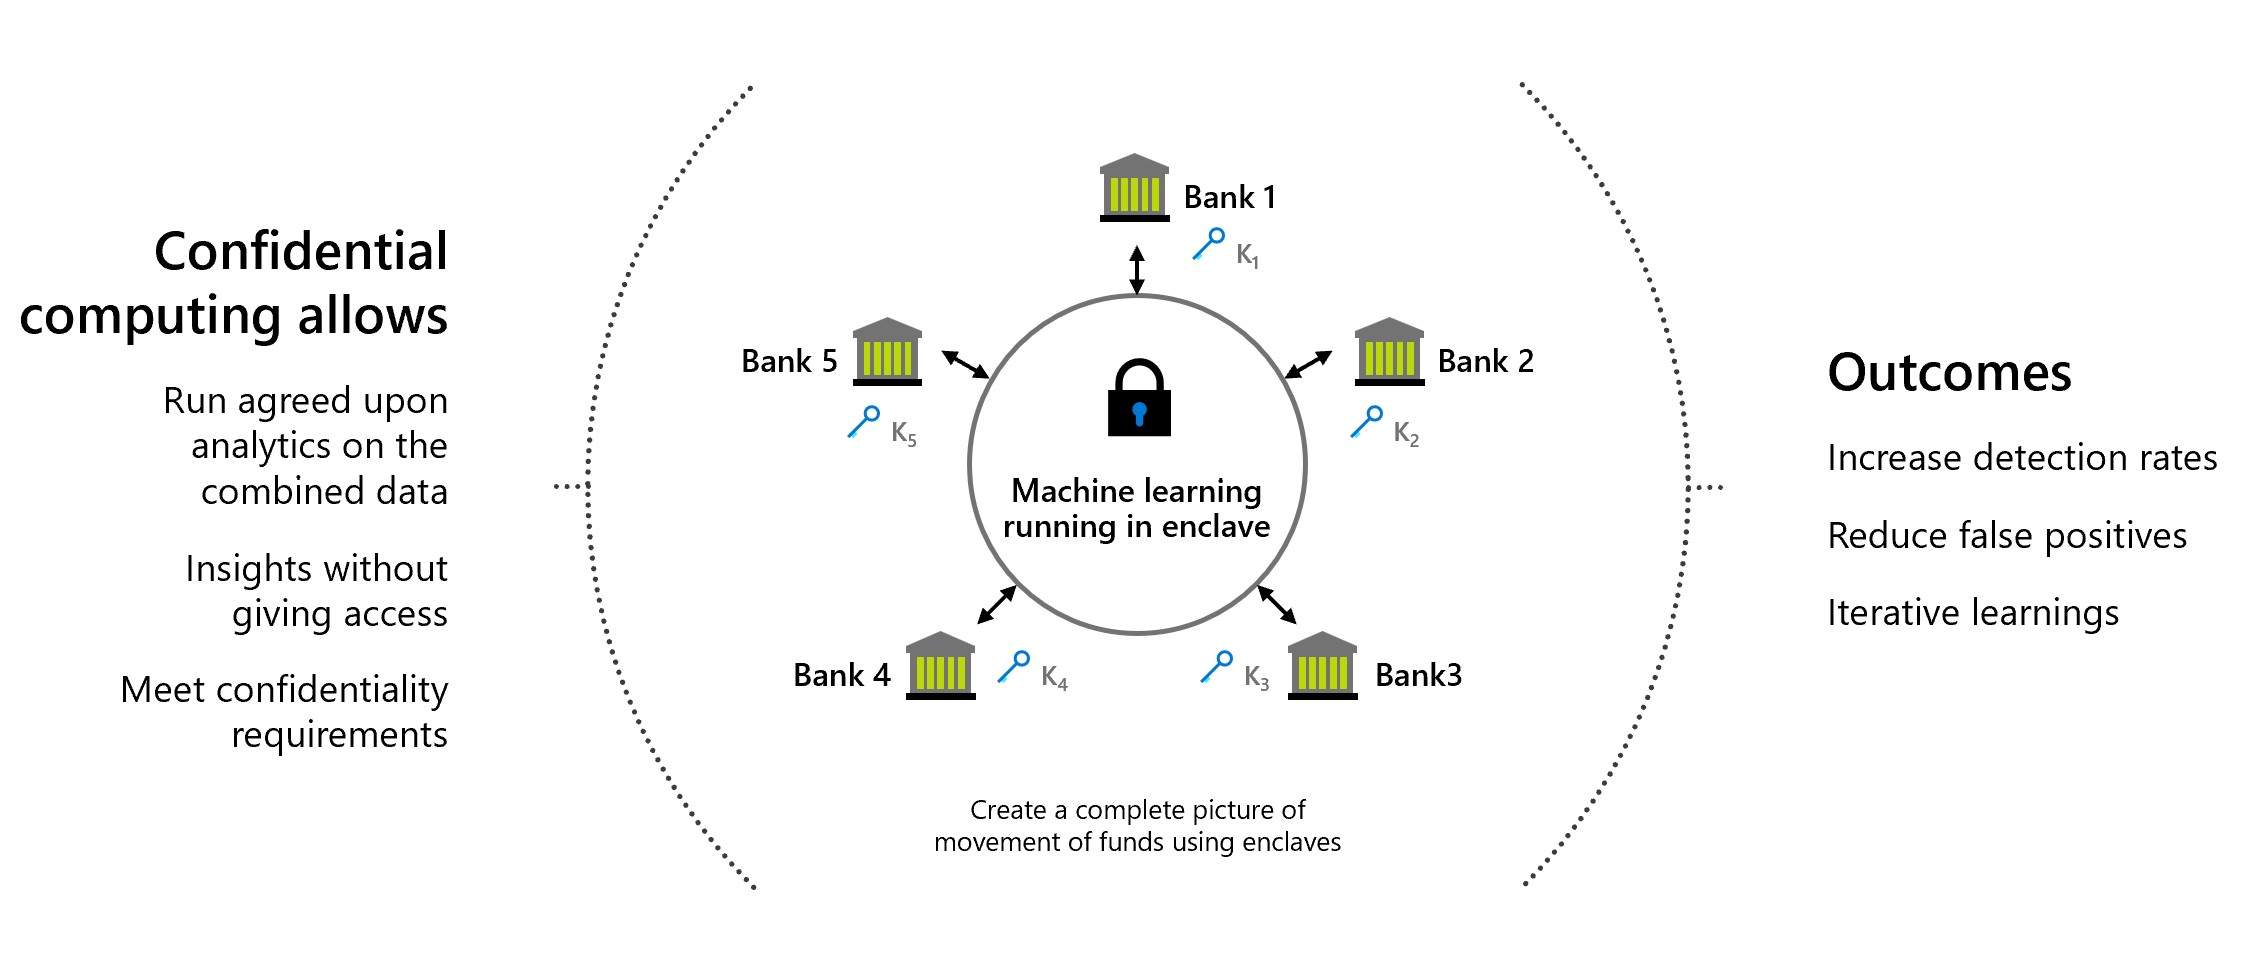
\includegraphics[width=\linewidth]{figures/mpc-banking.png}}
\caption{Secure Multi-Party Computation in Banking. Source: \cite{azure_mpc}}
\label{fig:mpc_banking}
\end{figure}

\begin{figure}[H]
\centerline{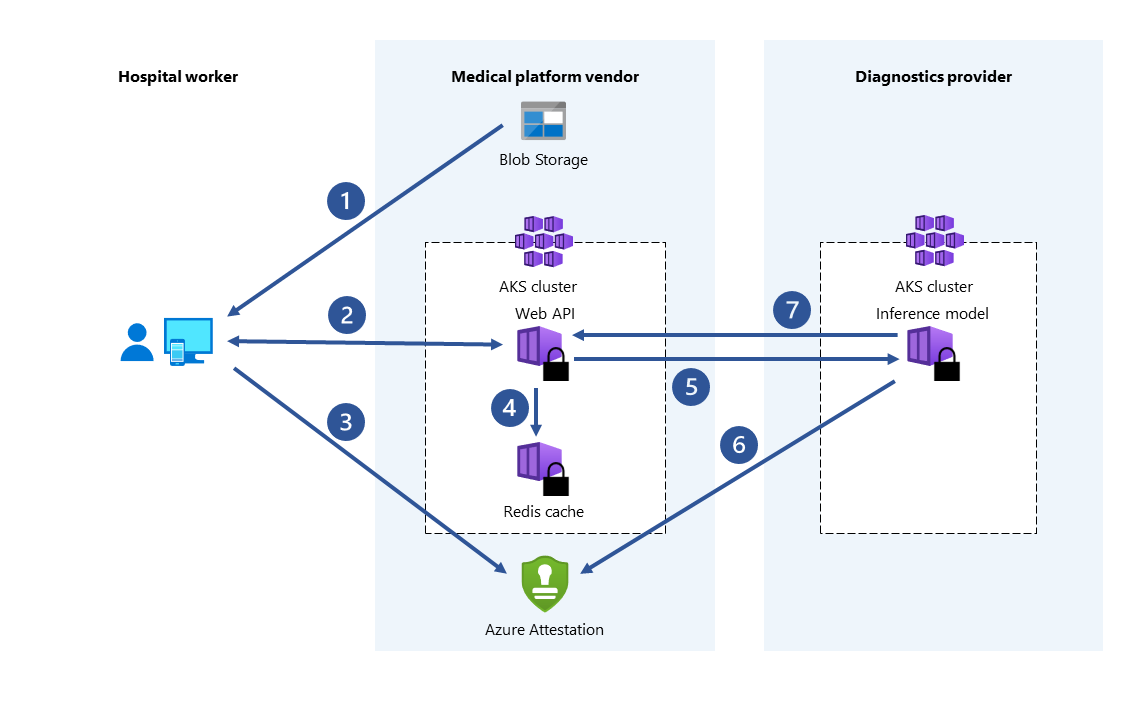
\includegraphics[width=\linewidth]{figures/confidential_healthcare.png}}
\caption{confidential healthcare system. Source: \cite{azure_mpc}}
\label{fig:mpc_banking}
\end{figure}

B. Privacy-Preserving AI
Machine learning models often require access to sensitive datasets for training or inference. 
Confidential computing enables models to operate on encrypted data within TEEs, ensuring that 
neither the data nor the model parameters are exposed. This is particularly valuable in healthcare, 
where patient data confidentiality is paramount. Platforms like BeeKeeperAI facilitate secure 
clinical algorithm development by providing a zero-trust environment for data stewards and AI 
developers \cite{beekeeper_ai}.

C. Secure Edge Computing
Edge devices operating in untrusted environments, such as retail stores or autonomous vehicles, 
benefit from on-device computation that guarantees data integrity and confidentiality. By 
embedding TEEs in edge hardware, organizations can ensure that sensitive data is processed 
securely, even in remote or physically insecure locations. This approach is crucial for 
applications requiring real-time data analysis and decision-making.

D. Intellectual Property Protection
Organizations can safeguard proprietary algorithms and business logic by executing them within 
TEEs \cite{ibm}. This ensures that intellectual property remains confidential, even when deployed in shared 
or public cloud environments. Industries such as finance and pharmaceuticals leverage this 
capability to protect sensitive computations from insider threats and external attacks \cite{anjuna_ip}.

E. Smart buildings utilize IoT devices to monitor occupancy, energy usage, 
and environmental conditions. These devices often collect sensitive data, such as CCTV footage 
or badge scans, which can be personally identifiable. Confidential computing enables processing 
this data within Trusted Execution Environments (TEEs), ensuring privacy and compliance with 
regulations like GDPR \cite{azure_mpc}.

\begin{figure}[H]
\centerline{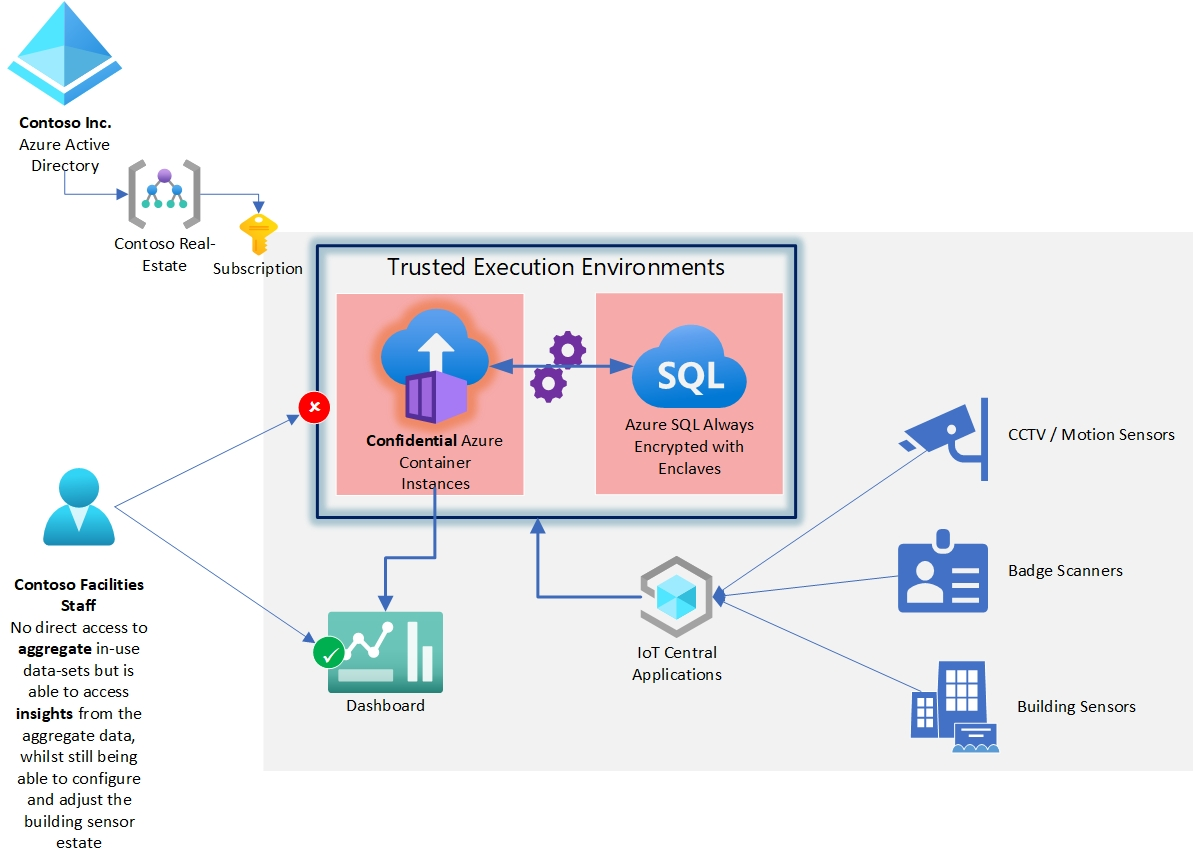
\includegraphics[width=\linewidth]{figures/iot-sensors.jpg}}
\caption{Privacy-Preserving Data Processing in Smart Buildings. Source: \cite{azure_mpc}}
\label{fig:smart_building_privacy}
\end{figure}

F. Manufacturing processes often involve proprietary designs and techniques. 
When outsourcing production, there's a risk of intellectual property (IP) theft. 
By leveraging confidential computing, manufacturers can run sensitive computations within TEEs, 
ensuring that their IP remains protected even in untrusted environments 
\cite{azure_mpc}.

\begin{figure}[H]
\centerline{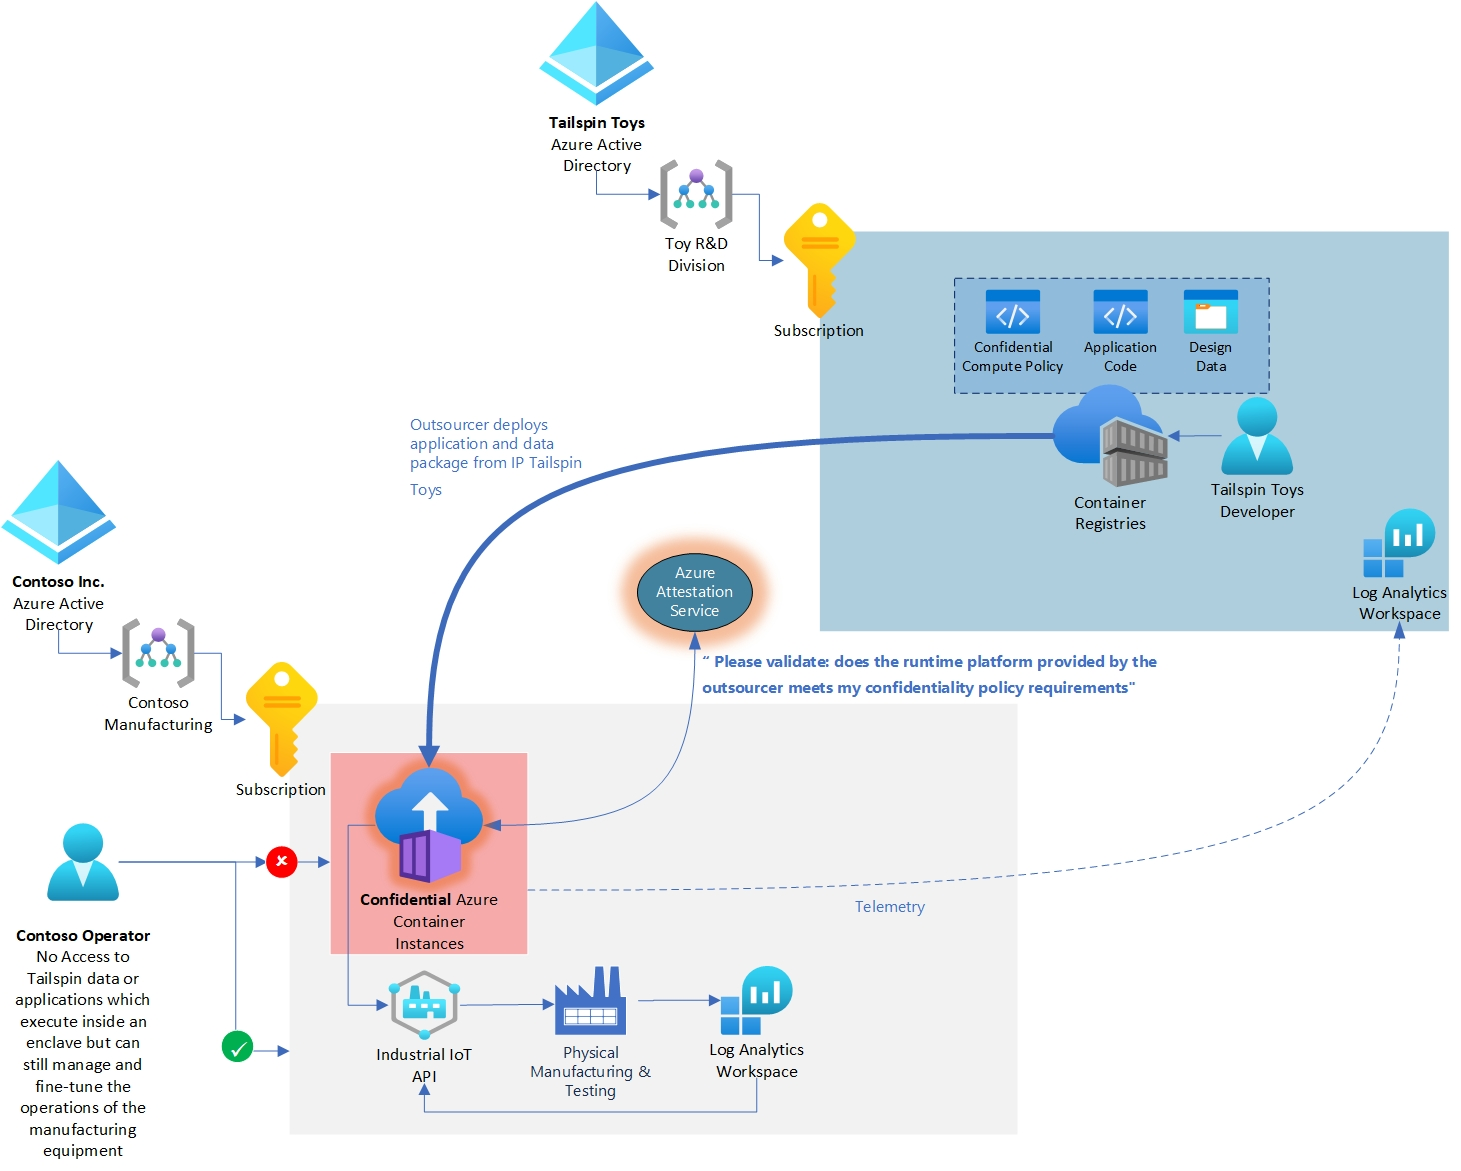
\includegraphics[width=\linewidth]{figures/manufacturing-ip-protection.jpg}}
\caption{Securing Manufacturing IP with Confidential Computing. Source: \cite{azure_mpc}}
\label{fig:manufacturing_ip_protection}
\end{figure}


\section{Case Studies}
\subsection{Accelerating Healthcare AI Development with BeeKeeperAI}

The University of California, San Francisco's (UCSF) Center for Digital Health Innovation (CDHI) 
has developed BeeKeeperAI, a platform that leverages Intel® Software Guard Extensions (SGX) and 
Microsoft Azure Confidential Computing to facilitate the secure validation of clinical AI 
algorithms \cite{fortanix}. This approach enables algorithm developers to validate their models against sensitive 
healthcare data without exposing patient information or intellectual property. By utilizing 
secure enclaves, BeeKeeperAI ensures that both data and algorithms remain confidential throughout 
the validation process, significantly reducing the time and cost associated with developing 
clinical AI solutions \cite{intel}.

\subsection{Enhancing Financial Services Security through AMD and Google Cloud Collaboration}

In a joint effort to bolster the security of confidential computing technologies, Google Cloud and 
AMD conducted a comprehensive audit of AMD's Secure Encrypted Virtualization-Secure Nested Paging 
(SEV-SNP) firmware. This collaboration involved Google's Project Zero and AMD's firmware team, 
aiming to identify and mitigate potential vulnerabilities in AMD's confidential computing stack. 
The audit led to the discovery and remediation of several security issues, reinforcing the 
integrity of AMD's SEV-SNP technology and setting a precedent for transparency and cooperation 
in enhancing cloud security \cite{wired}.

\section{Limitations and Challenges}
Despite its promise, confidential computing still faces key limitations:

• Hardware availability: Not all cloud instance types support TEEs, and they may incur 
additional costs.

• Performance penalties: Intel SGX enclaves are limited in memory (~128MB usable by default), 
and entering/exiting enclaves adds latency \cite{costan2016intel}. AMD SEV provides larger memory scopes but also 
incurs I/O overhead.

• Complex development model: Developers must often use constrained SDKs and modify applications 
to run in enclaves. Debugging is also restricted due to security constraints.

• Side-channel vulnerabilities: Attacks such as Foreshadow and Spectre exploit microarchitectural 
features to leak secrets, even from secure enclaves \cite{van2018foreshadow}.

These challenges must be addressed before Confidential Computing can see widespread production 
deployment.

\section{Conclusion}
Confidential Computing is a promising development in cloud security, extending protection to data 
in use through hardware-based TEEs. While current technologies such as Intel SGX, AMD SEV, and ARM 
TrustZone offer solid foundations, there are still usability, performance, and security challenges 
to overcome.

We recommend further work in:

• Cross-platform APIs for enclave development

• Improved developer tooling and SDKs

• Research into secure multi-party computation on cloud-scale platforms

• Mitigation of side-channel attacks through hardware and compiler-level innovations

Confidential Computing is not a silver bullet, but as part of a larger defense-in-depth strategy, 
it offers strong guarantees for sensitive cloud workloads.

\bibliographystyle{IEEEtran}
\bibliography{references}

\end{document}
